\documentclass[tikz, border=1mm]{standalone}
\usetikzlibrary{arrows, shapes.gates.logic.US, calc}
\begin{document}
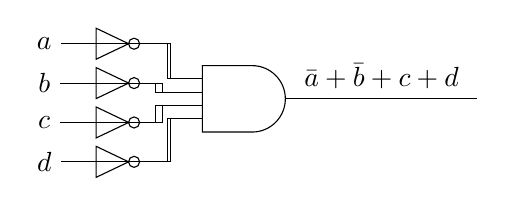
\begin{tikzpicture}
    \node (x) at (0, 1.5) {$a$};
    \node (y) at (0, 1) {$b$};
    \node (z) at (0, 0.5) {$c$};
    \node (w) at (0, 0) {$d$};

    \node[not gate US, draw] at ($(x) + (0.8, 0)$) (notx) {};
    \node[not gate US, draw] at ($(y) + (0.8, 0)$) (noty) {};
    \node[not gate US, draw] at ($(z) + (0.8, 0)$) (notz) {};
    \node[not gate US, draw] at ($(w) + (0.8, 0)$) (notw) {};
    
    \node[and gate US, draw, rotate=0, logic gate inputs=nnnn] at ($(w) + (2.5, 0.8)$) (xory) {};

    \draw (x) -- (notx.input);
    \draw (y) -- (noty.input);
    \draw (z) -- (notz.input);
    \draw (w) -- (notw.input);

    \draw (notx.output) -- ([xshift=0.35cm]notx.output) |- (xory.input 1);
    \draw (noty.output) -- ([xshift=0.2cm]noty.output) |- (xory.input 2);
    \draw (notz.output) -- ([xshift=0.2cm]notz.output) |- (xory.input 3);
    \draw (notw.output) -- ([xshift=0.35cm]notw.output) |- (xory.input 4);

    \draw (x) -| ($(x) + (1.6, -0.4)$) |- (xory.input 1);
    \draw (y) -| ($(y) + (1.5, -0.1)$) |- (xory.input 2);
    \draw (z) -| ($(z) + (1.5, 0.2)$) |- (xory.input 3);
    \draw (w) -| ($(w) + (1.6, 0.3)$) |- (xory.input 4);

    \draw (xory.output) -- node[above]{$\bar a + \bar b + c+d$} ($(xory) + (3, 0)$);
\end{tikzpicture}

  

                
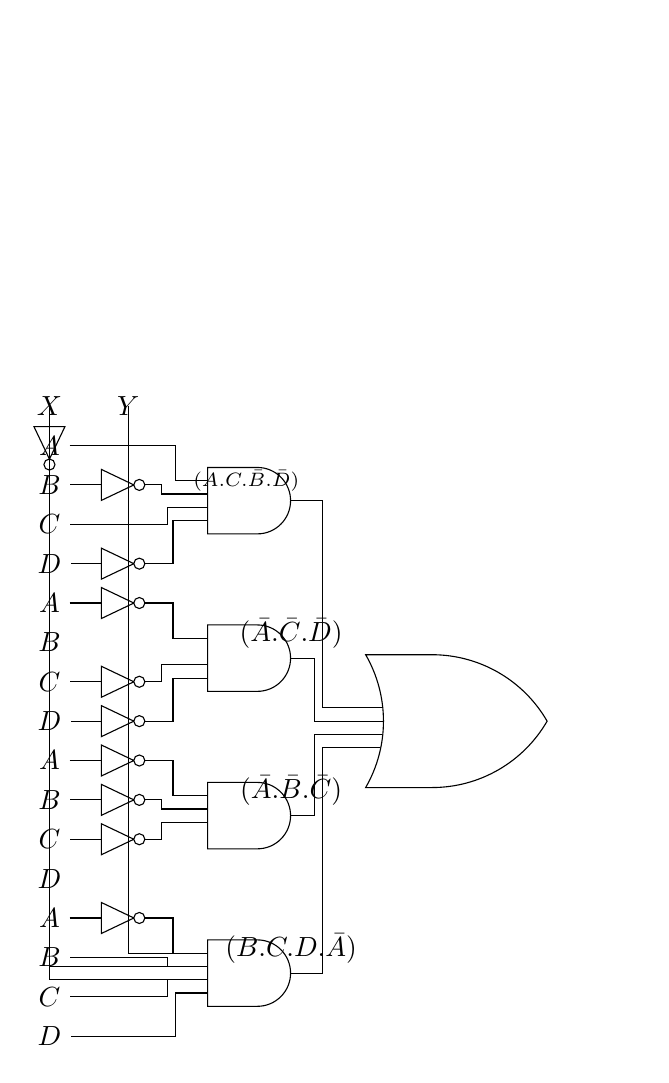
\begin{tikzpicture}
          
               \node (x0) at (0, 0*2+1.5) {$A$};
               \node (y0) at (0, 0*2+1) {$B$};
               \node (z0) at (0, 0*2+0.5) {$C$};
               \node (w0) at (0, 0*2+0) {$D$};
               \node (x) at (0, 4*2) {$X$};
               \node (y) at (1, 4*2) {$Y$};
             
               \node[and gate US, draw, rotate=0, logic gate inputs=nnnn] at ($(w0) + (2.5, 0.8)$) (xory0) {};
               \draw (xory0.output)  node[above]{$(B.C.D.\bar A)$} ($(xory0) + (2, 0)$);
               
               %% X'
               \node[not gate US, draw] at ($(x0) + (0.8, 0)$) (notx0) {};
               \draw (x0) -- (notx0.input);
               \draw (notx0.output) -- ([xshift=0.35cm]notx0.output) |- (xory0.input 1);
                 
               %% Y
               \draw (y0) -| ($(y0) + (1.5, -0.1)$) |- (xory0.input 2);
               \node[not gate US, draw, rotate=270] at ($(x) + (0, -0.4)$) (notx) {};
               \draw (x) -- (notx.input);               
               \draw (y) -| ($(y) + (0, -0.1)$) |- (xory0.input 1);
               \draw (x) -| ($(x) + (0, 0)$) |- (xory0.input 2);
               \draw (notx.output) -| ($(notx.output) + (0, 0)$) |- (xory0.input 3);
           
               %%Z
               \draw (z0) -| ($(z0) + (1.5, 0.2)$) |- (xory0.input 3);
               %%W
               \draw (w0) -| ($(w0) + (1.6, 0.3)$) |- (xory0.input 4);
                   
               \node (x1) at (0, 1*2+1.5) {$A$};
               \node (y1) at (0, 1*2+1) {$B$};
               \node (z1) at (0, 1*2+0.5) {$C$};
               \node (w1) at (0, 1*2+0) {$D$};
             
               \node[and gate US, draw, rotate=0, logic gate inputs=nnnn] at ($(w1) + (2.5, 0.8)$) (xory1) {};
               \draw (xory1.output)  node[above]{$(\bar A.\bar B.\bar C)$} ($(xory1) + (2, 0)$);
               
               %% X'
               \node[not gate US, draw] at ($(x1) + (0.8, 0)$) (notx1) {};
               \draw (x1) -- (notx1.input);
               \draw (notx1.output) -- ([xshift=0.35cm]notx1.output) |- (xory1.input 1);
               
               %Y'
               \node[not gate US, draw] at ($(y1) + (0.8, 0)$) (noty1) {};
               \draw (y1) -- (noty1.input);    
               \draw (noty1.output) -- ([xshift=0.2cm]noty1.output) |- (xory1.input 2);
             
               %%Z'
               \node[not gate US, draw] at ($(z1) + (0.8, 0)$) (notz1) {};
               \draw (z1) -- (notz1.input);
               \draw (notz1.output) -- ([xshift=0.2cm]notz1.output) |- (xory1.input 3);
                     
               \node (x2) at (0, 2*2+1.5) {$A$};
               \node (y2) at (0, 2*2+1) {$B$};
               \node (z2) at (0, 2*2+0.5) {$C$};
               \node (w2) at (0, 2*2+0) {$D$};
             
               \node[and gate US, draw, rotate=0, logic gate inputs=nnnn] at ($(w2) + (2.5, 0.8)$) (xory2) {};
               \draw (xory2.output)  node[above]{$(\bar A.\bar C.\bar D)$} ($(xory2) + (2, 0)$);
               
               %% X'
               \node[not gate US, draw] at ($(x2) + (0.8, 0)$) (notx2) {};
               \draw (x2) -- (notx2.input);
               \draw (notx2.output) -- ([xshift=0.35cm]notx2.output) |- (xory2.input 1);
               
               %%Z'
               \node[not gate US, draw] at ($(z2) + (0.8, 0)$) (notz2) {};
               \draw (z2) -- (notz2.input);
               \draw (notz2.output) -- ([xshift=0.2cm]notz2.output) |- (xory2.input 3);
             
               %%W
               \node[not gate US, draw] at ($(w2) + (0.8, 0)$) (notw2) {};
               \draw (w2) -- (notw2.input);
               \draw (notw2.output) -- ([xshift=0.35cm]notw2.output) |- (xory2.input 4);
                     
               \node (x3) at (0, 3*2+1.5) {$A$};
               \node (y3) at (0, 3*2+1) {$B$};
               \node (z3) at (0, 3*2+0.5) {$C$};
               \node (w3) at (0, 3*2+0) {$D$};
             
               \node[and gate US, draw, rotate=0, logic gate inputs=nnnn] at ($(w3) + (2.5, 0.8)$) (xory3) {};
               \draw (xory3) node[above]{\scriptsize $(A.C.\bar B.\bar D)$} ($(xory3) + (5, 6)$);
               %% X
               \draw (x3) -| ($(x3) + (1.6, -0.4)$) |- (xory3.input 1);
               
               %Y'
               \node[not gate US, draw] at ($(y3) + (0.8, 0)$) (noty3) {};
               \draw (y3) -- (noty3.input);    
               \draw (noty3.output) -- ([xshift=0.2cm]noty3.output) |- (xory3.input 2);
             
               %%Z
               \draw (z3) -| ($(z3) + (1.5, 0.2)$) |- (xory3.input 3);
           
               %%W
               \node[not gate US, draw] at ($(w3) + (0.8, 0)$) (notw3) {};
               \draw (w3) -- (notw3.input);
               \draw (notw3.output) -- ([xshift=0.35cm]notw3.output) |- (xory3.input 4);
             
              \node[or gate US, draw, rotate=0, logic gate inputs=nnnnnnnnn] at (5, 4) (xory) {};
             \draw (xory0.output) -- ([xshift=0.4cm]xory0.output) |- (xory.input 7);
             \draw (xory1.output) -- ([xshift=0.3cm]xory1.output) |- (xory.input 6);
             \draw (xory2.output) -- ([xshift=0.3cm]xory2.output) |- (xory.input 5);
             \draw (xory3.output) -- ([xshift=0.4cm]xory3.output) |- (xory.input 4);
   \end{tikzpicture}
                
     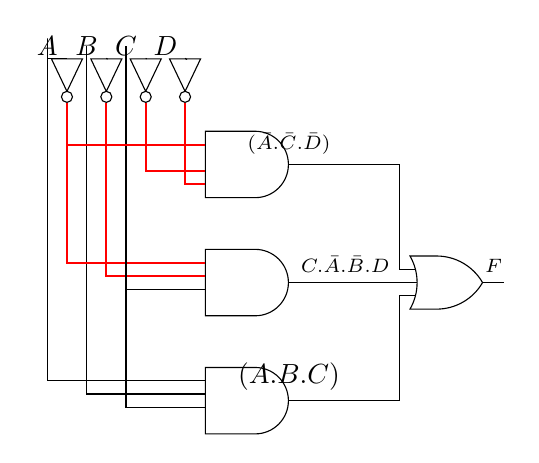
\begin{tikzpicture}
\node (x) at (0, 3*1.5) {$A$};
            \node (y) at (0.5, 3*1.5) {$B$};
            \node (z) at (1, 3*1.5) {$C$};
            \node (w) at (1.5, 3*1.5) {$D$};
            \node[not gate US, draw, rotate=270] at ($(x) + (0.25, -0.3)$) (notx) {};
            \draw (x) -| ($(x) + (0, 0.1)$) |- (notx.input); 
            \node[not gate US, draw, rotate=270] at ($(y) + (0.25, -0.3)$) (noty) {};
            \draw (y) -- (noty.input); 
            \node[not gate US, draw, rotate=270] at ($(z) + (0.25, -0.3)$) (notz) {};
            \draw (z) -- (notz.input);
            \node[not gate US, draw, rotate=270] at ($(w) + (0.25, -0.3)$) (notw) {};
            \draw (w) -- (notw.input);
                
           
            \node[and gate US, draw, rotate=0, logic gate inputs=nnnn] at (2.5, 0*1.5) (xandy0) {};
            \draw (xandy0.output)  node[above]{$(A.B.C)$} ($(xandy0) + (2, 0)$);
            %% X
            \draw (x) -| ($(x) + (0, 0)$) |- (xandy0.input 1);
              
            %% Y
            \draw (y) -| ($(y) + (0, 0)$) |- (xandy0.input 2);
        
            %%Z
            \draw (z) -| ($(z) + (0, 0)$) |- (xandy0.input 3);
                
           
            \node[and gate US, draw, rotate=0, logic gate inputs=nnnn] at (2.5, 1*1.5) (xandy1) {};
            \draw (xandy1.output) -- node[above]{\scriptsize$C.\bar A.\bar B.D$} ($(xandy1) + (2, 0)$);
            
            %% X'

            \draw  [line width=0.25mm,   red] (notx.output) -- ([xshift=0cm]notx.output) |- (xandy1.input 1);
            
            %Y'

            \draw [line width=0.25mm,   red] (noty.output) -- ([xshift=0cm]noty.output) |- (xandy1.input 2);
          
            %%Z
            \draw (z) -| ($(z) + (0, 0)$) |- (xandy1.input 3);
                
           
            \node[and gate US, draw, rotate=0, logic gate inputs=nnnn] at (2.5, 2*1.5) (xandy2) {};
            \draw (xandy2.output)  node[above]{\scriptsize$(\bar A.\bar C.\bar D)$} ($(xandy2) + (2, 0)$);
            
            %% X'

            \draw  [line width=0.25mm,   red] (notx.output) -- ([xshift=0cm]notx.output) |- (xandy2.input 1);
            
            %%Z'

            \draw [line width=0.25mm,   red] (notz.output) -- ([xshift=0cm]notz.output) |- (xandy2.input 3);
          
            %%W

            \draw [line width=0.25mm,   red] (notw.output) -- ([xshift=0cm]notw.output) |- (xandy2.input 4);
          \node[or gate US, draw, rotate=0, logic gate inputs=nnn] at (5, 3*0.5) (xory) {};
            \draw (xory.output) -- node[above]{\scriptsize$F$} ($(xory) + (0.8, 0)$);
\draw (xandy0.output) -- ([xshift=1.40cm]xandy0.output) |- (xory.input 3);

\draw (xandy1.output) -- ([xshift=1.35cm]xandy1.output) |- (xory.input 2);

\draw (xandy2.output) -- ([xshift=1.40cm]xandy2.output) |- (xory.input 1);


      \end{tikzpicture}           
        \end{document}
